\documentclass[twocolumn,nofootinbib]{revtex4}
%\usepackage{amsmath}
%\usepackage{iopams}
\usepackage{amsmath}
\usepackage{hyperref}
\usepackage{amssymb}
\usepackage{color}
\usepackage{epsfig}
\usepackage{latexsym}
\usepackage{tensor}
%\usepackage{wasysym}
\usepackage{comment}
%\usepackage{graphicx}
%\usepackage{psfrag}


\newcommand{\gw}{gravitational wave }
\newcommand{\gws}{gravitational waves }
\newcommand{\subgw}{_{\textrm{\scriptsize{GW}}}}
\newcommand{\ee}[1]{\!\times\!10^{#1}}
\newcommand{\prob}{{\rm Pr}}
\newcommand{\grbrate}{{{\mathcal R}_{\mathrm{grb}}}}
\newcommand{\cbcrate}{{{\mathcal R}}}
\newcommand{\diff}{{\mathrm d}}
\newcommand{\rhostar}{{\rho^*}}

\begin{document}

\title{Constraints On Short, Hard Gamma-Ray Burst Beaming Angles From
Gravitational Wave Observations}
\author{James Clark and Ik Siong Heng}
\date{\today}

\begin{abstract}
Apologies in advance for inconsistent conditioning statements in probabilities
\dots
\end{abstract}

\maketitle

\section{Introduction}

It is common in the literature to draw inferences on the rate of binary
coalescence $\cbcrate$, given some estimate for the beaming angle $\theta$ and
the observed rate of sGRBs $\grbrate$.  In this work, we investigate what
statements can \emph{currently} be made on the beaming angle itself using the
upper limits placed on $\cbcrate$ from all-sky, all-time \gw searches and
explore the potential for direct inference of sGRB  beaming angles in the
advanced detector era.

\section{Limits On sGRB Beaming Angles From Past Gravitational Wave Searches}

\subsection{Complete Sky-Coverage \& Known Observed GRB Rate}
Assuming all-sky Gamma-ray coverage and that all compact binary coalescence
events result in a short-hard gamma-ray burst, the rate of binary coalescences
is,
%
\begin{equation}\label{eq:rate2angle}
\cbcrate=\frac{\grbrate}{1-\cos \theta},
\end{equation}
where $\theta$ is the beaming angle of the outflow from the GRB and $\grbrate$
is the \emph{observed} sGRB rate.  We take
$\grbrate=10$\,Gpc$^{-3}$\,yr$^{-1}$~\cite{nakar-2007,Dietz11}.
%
Inferences of the GRB beaming angle may then be drawn from the posterior
probability density on the beaming angle, related to that on the rate posterior
via,
%
\begin{eqnarray}
p(\theta|D,I) & = & p(\cbcrate|D,I) \left|\frac{\diff \cbcrate}{\diff
\theta}\right| \\
\label{eq:rate2angleProb}
& = & p(\cbcrate|D,I) \times \left| \frac{\grbrate\sin\theta}{(1-\cos \theta)^2} \right|,
\end{eqnarray}
%
where the Jacobian is computed from equation~\ref{eq:rate2angle}, $D$ represents
our \gw observations and we explicitly include the conditioning information $I$
to remind us of the assumptions in the analysis.

Following~\cite{Biswas09,BradyFairhurst08}, the posterior on the binary
coalescence rate may be determined from the loudest event in the \gw
analysis.  Specifically, for a foreground event rate due to  binary coalescence
$\cbcrate$, the probability of obtaning no events with ranking statistic $\rho$
greater than the observed loudested event $\rhostar$ is,
%
\begin{equation}
P_F(\rhostar | \cbcrate, C_L, T) = e^{-\cbcrate C_L(\rhostar) T},
\end{equation}
%
where $C_L(\rhostar)$ is the total luminosity to which the search is sensitive
and $T$ is the duration of the search.  The overall probability of obtaining
no events with ranking statistic $\rho>\rhostar$ is the product of obtaining
no such events from foreground \emph{and} the probability of obtaining no such
events from the background in the detector, denoted $P_B(\rhostar)$,
%
\begin{equation}
P(\rhostar|\cbcrate,I) = P_B(\rhostar|I)e^{-\cbcrate C_L(\rhostar) T}
\end{equation}
%
Using a uniform prior on $\cbcrate$ and inverting the overall probability with
Bayes' theorem, we arrive at,
%
\begin{equation}\label{eq:loudestEventPosterior}
p(\cbcrate | C_L({\rhostar}, T, \Lambda) \propto p(\cbcrate) \left[ \frac{1+\Lambda
C_L(\rhostar) T}{1+\Lambda}\right] e^{-\cbcrate C_L(\rhostar) T}
\end{equation}
%
where $p(\cbcrate)$ is the prior probability distribution on the rate.  The
quantity $\hat{\Lambda}$ measures the relative probability of detecting an event
with ranking statistic $x$ due to \gws versus the probability of an equally loud
event arising in the background distribution.  The reader is directed to
section\,3 of~\cite{BradyFairhurst08} for a full discussion of this quanitity.

Now, recall that our objective is to derive a posterior on the jet angle
$\theta_j$ from the posterior on the rate of binary coalescence.  It is
straightforward to reconstruct the rate posterior from the published rate upper
limits: we simply require the value of $\Lambda$ and the product
$C_L T$.  
%
%To find this, note that the upper limit on the
%rate for confidence level $\alpha$ is by solving,
%
%\begin{equation}
%\alpha = \sideset{}{_0^{\cbcrate_{\alpha}}}\int p(\cbcrate | C_L(\rhostar), T, \Lambda )~\diff \cbcrate \nonumber
%\end{equation}
%
%for $\cbcrate_{\alpha}$.  
Assuming a uniform prior on the rate $\cbcrate$ and
the posterior given by equation~\ref{eq:loudestEventPosterior}, the upper limit
is given by equation 21 from~\cite{BradyFairhurst08}:
\begin{equation}
1-\alpha =  e^{-\cbcrate_{\alpha} C_L(\rhostar)T)}
\left[ 
1+ \left(\frac{\Lambda}{1+\Lambda}\right) \cbcrate_{\alpha} T C_L(\rhostar)
\right ]
\label{eq:rateIntegral}
\end{equation}
%
For now, let us focus attention on the interpretation of upper limits
from past \gw analyses.  No \gw signal has been observed and the loudest
event is umabiguously due to background noise fluctuations.  That is, the limit
in which $\Lambda \rightarrow 0$.  In this case, we simply have,
\begin{equation}
C_L(\rhostar)T = -\frac{\log(1-\alpha)}{\cbcrate_{\alpha}},
\end{equation}
and the value of $\cbcrate$ can be taken straight from the literature.  Note
that this procedure necessarily confines our jet angle inferences based on
progenitor systems for which the rate upper limits are available.  Given that
the binary coalesence rate limits are quoted for canonical binary neutron star
and neutron star-black hole systems, both plausible sGRB progenitors, this
simply means our inferences on the jet angle are specific to each system and
treated separately.

Using the most stringent 90\% confidence upper limit from \gw observations on the
rate of binary neutron star coalescences to date,
$\cbcrate^{90\%}_{{\rm bns}} = 1.3\times
10^{-4}$\,Mpc$^{-3}$yr$^{-1}$~\cite{S6lowmass}, gives $C_L(\rhostar)T=17712$.
Similarly, for NS-BH systems,  $\cbcrate^{90\%}_{{\rm nsbh}} = 3.1\times
10^{-5}$\,Mpc$^{-3}$yr$^{-1}$ gives $C_L(\rhostar)T=74277$.  The posteriors on
the rates, assuming these values and $\Lambda=0$, are shown in
figure~\ref{fig:reconstructedRatePosterior}.  

Figure~\ref{fig:jetPosterior} shows the resulting posterior on the GRB
beaming angle, using the transformation in equation~\ref{eq:rate2angleProb} and
our results so far.  \textcolor{red}{Informal}: To interpret this posterior and
hence obtain a limit on the range of possible beaming angles, we need to
consider the question we're asking.  I (James) think this should probably be,
`what is the smallest jet angle that produces a result consistent with our
observations?'.  That is, we want a \emph{lower} limit.  Why not the
\emph{largest} jet angle?  I think that would involve allowing infinitely small
angles which doesn't really make sense.  I can't quite put my finger on it,
though.

Now, the quantity of interest is the inferred \emph{lower}
limit on the jet angle~$\theta^{90\%}$:
%
\begin{equation}
0.9 = \int_{\theta^{90\%}}^{\infty}p(\theta | \cbcrate^{90\%})~\diff \theta
\end{equation}
%
This is indicated with the vertical red line in figure~\ref{fig:jetPosterior}.
We find $\theta^{90\%}=3.3^{\circ}$.


\begin{figure}
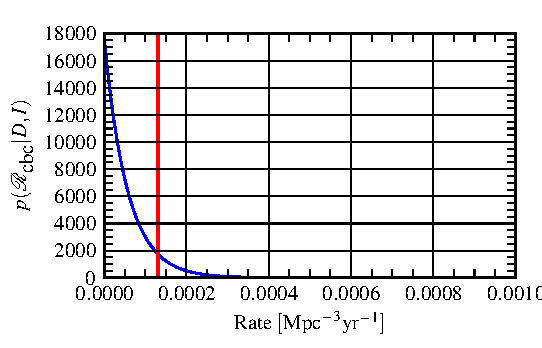
\includegraphics{rate_posterior_s6UL.eps}
\caption{Rate posterior for S6/VSR2,3 Low-mass Search For Compact Binary
Coalescence.\label{fig:reconstructedRatePosterior}}
\end{figure}

\begin{figure}
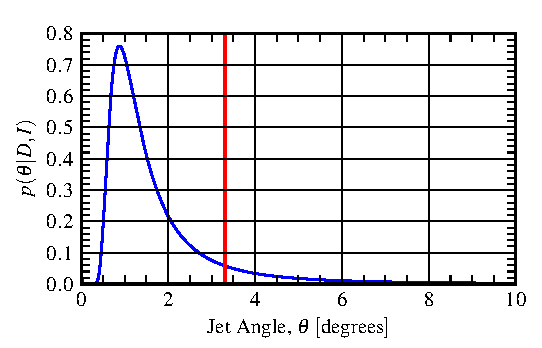
\includegraphics{jet_angle_posterior_s6UL.eps}
\caption{Jet angle posterior derived from S6/VSR2,3 Low-mass Search For Compact Binary
Coalescence posterior / upper limit on compact binary coalescence
rate.\label{fig:jetPosterior}}
\end{figure}

\subsection{Incomplete Sky-Coverage \& Unknown GRB Rate}
Marginalise over some stuff for the case of an `impure' GRB sample (unknown
fraction of CBCs).
\\

\subsection{Astrophysical Interpretation \& Comparison With Other Limits}
The comparison with other limits is straightforward.  I think it looks pretty
consistent with Dietz, Holtz etc (but should double check).

More importantly, however,  we've demonstrated how to get a limit on the beaming
angle.  That's all well and good but we need some astrophysical interpretation,
really.  The most obvious thing (to James) is that the beaming angle is really a
proxy for the Lorentz factor of the outflow (I think):
%
\begin{equation}
\theta \sim \frac{1}{\Gamma}.
\end{equation}
%
So, what \emph{physics} of the progenitor can we constrain with this?

\section{Inferences On Beaming Angles Expected From Future Detections}
I'm less sure how to address this but I could imagine having a) a mock result
based on the Big Dog or b) a collection of mock results for e.g., a measured
non-zero rate after x years of observation (say).  Anything here is going to be
pretty speculative since we don't know about satellites.  In fact, maybe this is
an opportunity to devise a simple figure of merit to state what sort of
sky-coverage is required in each of the timelines in the observing scenarios
document to measure the jet angle to some accuracy?

\section{Conclusion}

\bibliography{grb_beams}

\end{document}
